% !TEX program = xelatex
% !TEX encoding = UTF-8

\documentclass[11pt, a4paper]{article} % use larger type; default would be 10pt

\usepackage{fontspec} % Font selection for XeLaTeX; see fontspec.pdf for documentation
\defaultfontfeatures{Mapping=tex-text} % to support TeX conventions like ``---''
\usepackage{xunicode} % Unicode support for LaTeX character names (accents, European chars, etc)
\usepackage{xltxtra} % Extra customizations for XeLaTeX
\usepackage{tikz}
\usetikzlibrary{arrows,calc,patterns}

\setmainfont[Ligatures=TeX]{[EBGaramond-Regular.ttf]} % set the main body font (\textrm), assumes Charis SIL is installed
%\setsansfont{Deja Vu Sans}
\setmonofont[Ligatures=TeX]{[FiraCode-Regular.ttf]}

% other LaTeX packages.....
\usepackage{fullpage}
\usepackage[top=2cm, bottom=4.5cm, left=2.5cm, right=2.5cm]{geometry}
\usepackage{amsmath,amsthm,amsfonts,amssymb,amscd,systeme}
\usepackage{unicode-math}
\usepackage{cancel}
\geometry{a4paper} 
%\usepackage[parfill]{parskip} % Activate to begin paragraphs with an empty line rather than an indent
\usepackage{fancyhdr}
\usepackage{listings}
\usepackage{graphicx}
\usepackage{hyperref}
\usepackage{multicol}

\renewcommand\lstlistingname{Algorithm}
\renewcommand\lstlistlistingname{Algorithms}
\def\lstlistingautorefname{Alg.}
\lstdefinestyle{mystyle}{
    % backgroundcolor=\color{backcolour},   
    % commentstyle=\color{codegreen},
    % keywordstyle=\color{magenta},
    % numberstyle=\tiny\color{codegray},
    % stringstyle=\color{codepurple},
    basicstyle=\ttfamily\footnotesize,
    breakatwhitespace=false,         
    breaklines=true,                 
    captionpos=b,                    
    keepspaces=true,                 
    numbers=left,                    
    numbersep=5pt,                  
    showspaces=false,                
    showstringspaces=false,
    showtabs=false,                  
    tabsize=2
}
\lstset{style=mystyle}

\newcommand\course{6 - Матстатистика}
\newcommand\hwnumber{Домашня КР №2}             % <-- homework number
\newcommand\idgroup{ФІ-91}                
\newcommand\idname{Михайло Корешков}  

\usepackage[framemethod=TikZ]{mdframed}
\mdfsetup{%
	backgroundcolor = black!5,
}
\mdfdefinestyle{ans}{%
    backgroundcolor = green!5,
    linecolor = green!50,
    linewidth = 1pt,
}

\pagestyle{fancyplain}
\headheight 35pt
\lhead{\idgroup \\ \idname}
\chead{\textbf{\Large \hwnumber}}
\rhead{\course \\ \today}
\lfoot{}
\cfoot{}
\rfoot{\small\thepage}
\headsep 1.5em

\linespread{1.2}

\begin{document}

\section*{№1}
\begin{mdframed}
    $$n = 15$$
    $$\xi_i \sim Exp(\lambda) - iid$$

    Побудувати $0.95$-довірчий інтервал для 
    \begin{itemize}
        \item $M\xi_1$
        \item $\sqrt{D\xi_1}$
    \end{itemize}
\end{mdframed}

\subsection*{1.}

Перш за все зазначу, що $M\xi_i = \frac{1}{\lambda}$.

Let $T_1(\vec X) = \overline X$. Це змістовна та незміщена оцінка $M\xi_1$.
Хочемо привести цю статистику до відомого розподілу.

Зауважу що $\chi^2(n) \sim Gamma(\frac{n}{2}, 2)$.

Спочатку перетворю $\xi_i$ наступним чином:\\
Нехай $\eta_i = 2\lambda\xi_i$.
$F_\eta(x) = F_\xi(\frac{x}{2\lambda})$.
$f_\eta(x) = \frac{\lambda}{2\lambda} e^{-\frac{\lambda}{2\lambda}x} = \frac{1}{2}e^{-\frac{x}{2}}$.
Тобто 
$$2\lambda\xi_i = \eta_i \sim \exp(\frac{1}{2}) \sim \chi^2(2)$$.

Тоді 
$$2 \lambda \sum_i \xi_i \sim \chi^2(2n)$$ 
- отримали табличний розподіл.

Let $\gamma = 0.95$.
$$P\left(g_1 < 2 \lambda \sum_i \xi_i < g_2\right) = \gamma$$
$$P\left(\frac{g_1}{2\sum_i \xi_i} <  \lambda  < \frac{g_2}{2\sum_i \xi_i}\right) = \gamma$$
$$P\left(\frac{2\sum_i \xi_i}{g_2} <  \frac{1}{\lambda}  < \frac{2\sum_i \xi_i}{g_1}\right) = \gamma$$

Використовую центральний інтервал із площею $\gamma$, залишаючи ліворуч та праворуч 
інтервали із площами $\frac{1-\gamma}{2}$ кожен. 
Це відповідає
$$g_1 = F^{-1}_{\chi^2(2n)}\left(\frac{1-\gamma}{2}\right)$$ 
$$g_2 = F^{-1}_{\chi^2(2n)}\left(\frac{1+\gamma}{2}\right)$$ 

Отримали $\gamma$-довірчий інтервал 
$$\left(\frac{2\sum_i \xi_i}{g_2} ; \frac{2\sum_i \xi_i}{g_1}\right)$$

Обчислимо його у Python:
\begin{figure}[h]
    \centering
    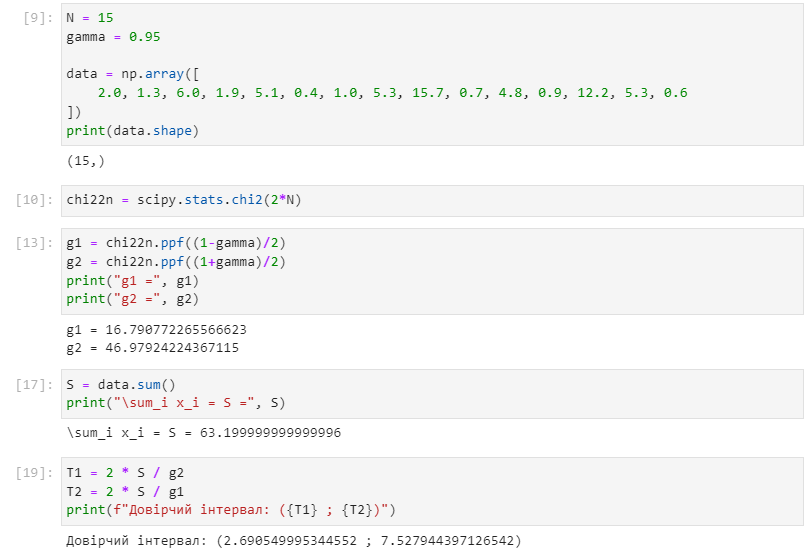
\includegraphics[width=0.9\textwidth]{img/task1.png}
\end{figure}

\begin{mdframed}[style=ans]
    Маємо $0.95$-довірчий інтервал для $M\xi_1$:
    $$P\left(2.69 < M\xi < 7.53\right) = 0.95$$
\end{mdframed}

\subsection*{2.}
Стандартне відхилення має вигляд
$$\sigma = \sqrt{D\xi_1} = \sqrt{\frac{1}{\lambda^2}} = \frac{1}{\lambda} = M\xi_1$$
Тобто підходить інтервал, знайдений в попередньому пункті
\pagebreak

\section*{№2}
\begin{mdframed}
    $$\xi_i \sim \mathcal{N}(\mu, \sigma^2) - iid;$$

    Знайти $0.95$-довірчі інтервали для $\mu$ та $\sigma$
\end{mdframed}

\subsection*{1. $\mu$}
Знаємо ОМП $\mu$:
$$T_1(\vec X) = \overline X$$

% \begin{mdframed}[backgroundcolor=blue!10]
%     $$L(\vec X, \mu, \sigma^2) = \exp\left\{ - \frac{1}{2\sigma^2}\sum_i (x_i-\mu)^2 \right\}$$
%     $$\frac{\partial}{\partial \mu} \ln L(\vec X, \mu, \sigma^2) = - \frac{1}{\sigma^2} \sum_i (x_i-\mu) = \frac{n}{\sigma^2}\left( \mu - \overline X \right) = 0$$
%     $$\implies \mu = \overline X$$
%     Дійсно ОМП
% \end{mdframed}

Знаємо ОМП $\sigma^2$:
$$T_2(\vec X) = S^2 = \frac{1}{n-1} \sum_{{i=1}}^n (X_i - \overline X)^2$$

Знаємо, що $$T = \frac{\overline{X} - \mu}{S \fracslash \sqrt{n}} \sim t(n-1)$$
- має розподіл Ст'юдента із $n-1$ степенями свободи - розподіл не залежить від $\mu$, $\sigma^2$.

Будуємо інтервал:
$$P(g_1 < T < g_2) = \gamma;$$
$$\text{let } g_1 = t_{n-1}^{-1}(\frac{1-\gamma}{2}); \; g_2 = t_{n-1}^{-1}(\frac{1+\gamma}{2})$$

З іншого боку
$$P(g_1 < T < g_2) = P(g_1 < \frac{\overline{X} - \mu}{S \fracslash \sqrt{n}} < g_2) = $$
$$= P(\frac{S}{\sqrt n} g_1 < \overline X - \mu < \frac{S}{\sqrt n}  g_2) = $$
$$= P(\overline X - \frac{S}{\sqrt n} g_2 < \mu < \overline X - \frac{S}{\sqrt n} g_1) = \gamma$$

Маємо інтервал для $\mu$.

\subsection*{2. $\sigma$}
Знаємо:
$$\zeta = \frac{n-1}{\sigma^2} S^2 \sim \chi^2(n-1)$$

Будуємо інтервал
$$P(g_1 < \zeta < g_2) = \gamma$$
$$\text{let } g_1 = F_{\chi^2(n-1)}^{-1}(\frac{1-\gamma}{2}); \; g_2 = F_{\chi^2(n-1)}^{-1}(\frac{1+\gamma}{2})$$

З іншого боку
$$P(g_1 < \frac{n-1}{\sigma^2} S^2 < g_2) = $$
$$= P(\frac{1}{g_2} < \frac{\sigma^2}{S^2(n-1)} < \frac{1}{g_1}) = $$
$$= P(\frac{S^2(n-1)}{g_2} < \sigma^2 < \frac{S^2(n-1)}{g_1}) = \gamma$$

Маємо інтервал для $\sigma^2$.

\subsection*{3. Обчислення}

\begin{figure}[h]
    \centering
    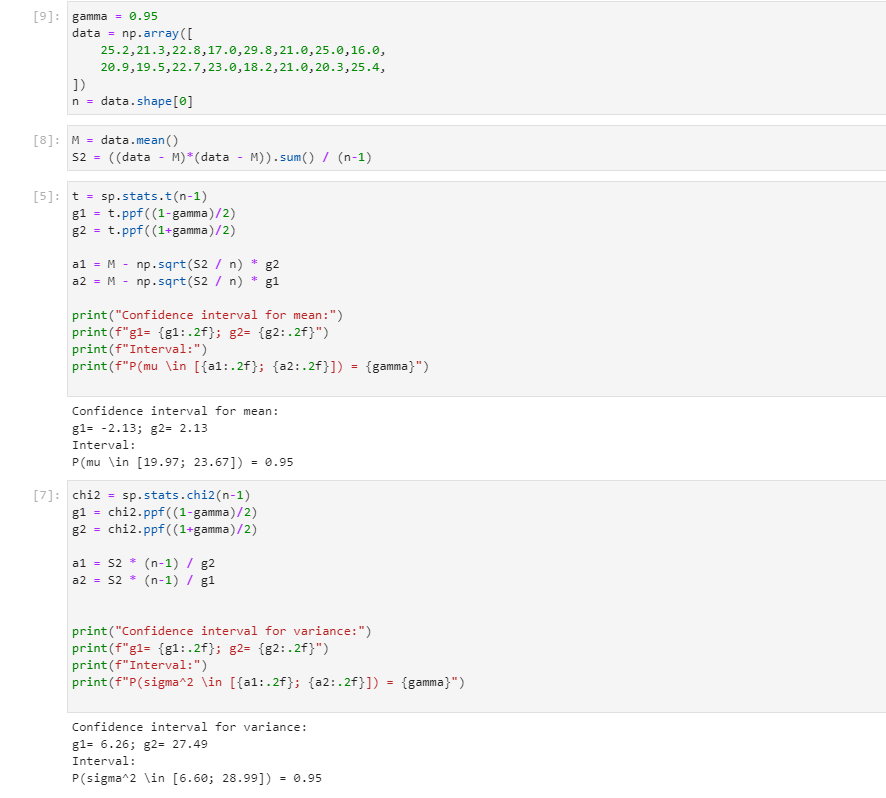
\includegraphics[width=1\textwidth]{img/task2.png}
\end{figure}

\begin{mdframed}[style=ans]
    $$P(\mu \in [19.97; 23.67]) = 0.95$$
    $$P(\sigma^2 \in [6.60; 28.99]) = 0.95$$
\end{mdframed}

\pagebreak

\section*{№3}

\begin{mdframed}
    $$X_i \sim \mathcal N (a,1)$$
    $$H0: \overline X \in [12.0; 12.6]$$
    $$H0 - \text{гіпотеза, що } \mu = 12.3$$
    $$H1: \overline X \notin [12.0; 12.6]$$
    $$H1 - \text{гіпотеза, що } \mu \ne 12.3$$
    $$n = 36$$
    $$\sigma = 1$$

    Обчислити рівень значущості критерію $\alpha$
\end{mdframed}

$$\overline X \sim \mathcal{N}(\mu, \frac{\sigma^2}{n})$$
$$\eta = \frac{\sqrt n (\overline X - \mu)}{\sigma} = 6(\overline X - 12.3) \sim \mathcal{N}(0,1)$$

$$\alpha(\mu) = P(H1 \;|\; H0)$$
$$\alpha(\mu) = P(\overline X \notin [12; 12.6] \; | \; \mu = 12.3) = $$
$$= P(\eta \notin [-0.3\cdot 6; 0.3 \cdot 6] \;|\; \mu = 12.3) = $$
$$= 1-\left(\Phi_{0,1}(1.8)-\Phi_{0,1}(-1.8)\right) = 2 - 2\Phi_{0,1}(1.8) \approx 0.0719$$

\begin{mdframed}[style=ans]
    Отже, рівень значущості має значення приблизно $0.072$
\end{mdframed}


\section*{№4}
\begin{mdframed}
    $$n = 10$$
    $$X_i \sim Exp(\lambda) - iid$$
    $$H0: \mu = 50000;\quad H1: \mu = 70000;\quad \alpha=0.05$$
\end{mdframed}

Найпотужнішим критерієм буде критерій Неймана-Пірсона, що визначається критичною областю виду 
$$\mathcal K = \left\{ \vec x :\; \frac{L_1}{L_0} \ge K \right\}$$
, де константа $K$ вибирається з умови заданої значущості:
$$P(\frac{L_1}{L_0} \ge K \;|\; H0) = \alpha$$

$$L(\vec x, \lambda) = \prod_{i=1}^n \lambda e^{-\lambda x_i} = \lambda^n e^{-\lambda n \overline X }$$

$$\frac{L_1}{L_0} = \left(\frac{\mu_0}{\mu_1}\right)^n e^{-n \overline X \left(\frac{1}{\mu_1} - \frac{1}{\mu_0}\right)} \ge K$$
$$e^{-n \overline X \left(\frac{1}{\mu_1} - \frac{1}{\mu_0}\right)} \ge K_1$$
$$+n \left(\overline X \left(\frac{1}{\mu_0} - \frac{1}{\mu_1}\right)\right) \ge K_2$$
$$\overline X \ge K_3$$
Тобто умова для вибору K має вигляд
$$P(\overline X \ge K \;|\; H0) = \alpha$$

$$\overline X \sim Gamma(n, n \lambda), \text{ як відома сума в.в.}$$
$$\eta = 2 n \lambda \overline X \sim Gamma(n, \frac{1}{2}) = \chi^2(2n)$$
або інакше, 
$$\eta = \frac{2n}{\mu} \overline X \sim \chi^2(2n)$$

$$P(\overline X \ge K \;|\; H0) = P(\eta \ge \frac{2n}{\mu_0} K) = 1 - P(\eta \le \frac{2n}{\mu_0} K) = \alpha$$
$$\frac{2n}{\mu_0} K = F_{\chi^2(2n)}^{-1}(1-\alpha) = 31.4$$
$$K = 78526$$

\begin{mdframed}[style=ans]
    Тобто маємо статистичний критерій для відкидання гіпотези H0:
    $$\overline X \ge 78526$$
\end{mdframed}
\pagebreak

\section*{№5}
\begin{mdframed}
    Розподіл Релея.
    $$f_\theta(x) = \frac{x}{\theta^2} e^{-\frac{x^2}{2\theta^2}}, \; x>0, \theta>0$$
    $$F_\theta(x) = 1 - e^{-\frac{x^2}{2\theta^2}}, \; x>0$$

    $$H_0: \theta = 1; \quad H_1: \theta > 1; \quad \alpha = 0.05$$
    Знайти найпотужніший критерій.
\end{mdframed}

Спочатку знайдемо $\varphi$:
$$L(\vec x, \theta) = \frac{1}{\theta^{2n}}\prod_{i=1}^n x_i \cdot e^{-\frac{1}{2\theta^2} \sum_i x_i^2}$$

Note: let $\theta_1 > \theta_0$
$$\varphi(\vec x) = \frac{L(\vec x, \theta_1)}{L(\vec x, \theta_0)} =  
\left(\frac{\theta_0}{\theta_1}\right)^{2n} \operatorname{exp}\left\{-\frac{\sum_i x_i^2}{2} \cdot \left(\frac{1}{\theta_1^2} - \frac{1}{\theta_0^2}\right)\right\}$$

Знайдемо критерій Неймана-Пірсона:
$$\varphi(\vec x) \ge K$$
$$\sum_{i=1}^n x_i^2 \ge K$$
Більше, а не менше, бо $\frac{1}{\theta_1^2} - \frac{1}{\theta_0^2} < 0$ за припущенням що $\theta_1 > \theta_0$.

Бачимо, що критерій Неймана-Пірсона не залежить від $\theta_1$, а значить, що найпотужніший критерій для заданих альтернатив 
існує та співпадає із цим. 
Шукаємо константу з умови значущості
$$P(\sum_{i=1}^n x_i^2 \ge K) = 0.05$$

Спочатку подивимось що це за розподіли
$$\xi = \sum_{i=1}^n X_i^2$$
$$\xi_i = X_i^2$$

$$P_\theta(\xi_i \le y) = P_\theta(X_i \le \sqrt{y}) = 1 - e^{-\frac{y}{2\theta^2}}$$
$$\theta = \theta_0 = 1$$
$$P_\theta(\xi_i \le y) = 1 - e^{-\frac{y}{2}}$$

Тобто
$$\xi_i \sim Exp(1\fracslash 2) = \chi^2(2)$$
А тоді $\xi$ має відомий розподіл
$$\xi \sim \chi^2(2n)$$

$$P(\sum_{i=1}^n x_i^2 \ge K) = 1 - F_{\chi^2_{2n}}(K) = 0.05$$
$$K = F^{-1}_{\chi^2_{2n}}(0.95)$$

Нехай $n\to \infty$.
$$\eta = \frac{\xi - 2n}{\sqrt{4n}} \sim \mathcal N(0,1)\quad (\text{бо } M\xi = 2n, D\xi = (2\cdot 2n)^2)$$
$$\eta = \frac{\xi-2n}{2\sqrt{n}}$$
$$P(\xi \ge K) = P(\frac{\xi-2n}{2\sqrt{n}} \ge \frac{K-2n}{2\sqrt{n}} ) = 0.05 = 1 - \Phi_{0,1}(\frac{K-2n}{2\sqrt{n}})$$
$$\Phi_{0,1}(\frac{K-2n}{2\sqrt{n}}) = 0.95$$
$$\frac{K-2n}{2\sqrt{n}} = 1.645$$
$$K = 2 \cdot 1.645 \cdot \sqrt{n} + 2n$$

\begin{mdframed}[style=ans]
    Найпотужнішим буде критерій
    $$\sum_{i=1}^n X_i^2 \ge 2 \cdot \Phi_{0,1}^{-1}(0.95) \cdot \sqrt{n} + 2n$$
\end{mdframed}

\pagebreak

\section*{№6}

\begin{mdframed}
    $$n=150; \quad \alpha = 0.05$$
    Гіпотеза $H_0$: розподіл $X_i$ є біноміальним $Bin(4,\theta)$
    $$P(X_i = k) = C_4^k \theta^k (1-\theta)^{n-k}, \; k=0,1,2,3,4$$ 
\end{mdframed}

Шукаємо ОМП для $\theta$
$$L(n_k, \theta) = \frac{n!}{n_0!n_1!n_2!n_3!n_4!} \prod_{i=0}^4 p_i^ni = $$
$$= C \cdot \theta^{4n_4 + 3n_3 + 2n_2 + n_1} \cdot (1-\theta)^{4n_0 + 3n_1 + 2n_2 + n_3}$$
$$\ln L = C + \ln \theta (4n_4 + 3n_3 + 2n_2 + n_1) + \ln (1-\theta) (4n_0 + 3n_1 + 2n_2 + n_3)$$
$$\frac{\partial}{\partial \theta} \ln L = \frac{4n_4 + 3n_3 + 2n_2 + n_1}{\theta} - \frac{4n_0 + 3n_1 + 2n_2 + n_3}{1-\theta} = 0$$
$$4n_4 + 3n_3 + 2n_2 + n_1 - \theta(4n_4 + 3n_3 + 2n_2 + n_1) - \theta(4n_0 + 3n_1 + 2n_2 + n_3) = 0$$
$$4n_4 + 3n_3 + 2n_2 + n_1 = 4n_0 + 4n_1 + 4n_2 + 4n_3 + 4n_4 = 4n$$

Маємо ОМП для $\theta$:
$$\hat \theta = \frac{4n_4 + 3n_3 + 2n_2 + n_1}{4n}$$
$$\hat \theta = \frac{233}{600} = 0.388$$

Використаємо критерій $\chi^2$ для перевірки складної параметричної гіпотези щодо вигляду поліноміального (тут - біноміального) розподілу.

$$p_k = C_4^k \theta^k (1-\theta)^{n-k}$$
$$p_0 = 0.140; \; p_1 = 0.355; \; p_2 = 0.339; \; p_3 = 0.134; \; p_4 = 0.023;$$
$$n_0 = 21; \; n_1 = 53; \; n_2 = 51; \; n_3 = 21; \; n_4 = 3;$$

$$\rho(\vec x) = \sum_{k=0}^4 \frac{(c_k - n_k)^2}{n_k} = 15.704$$
Відомо, що така $\rho \longrightarrow \chi^2(r-1-m)$,
де для біноміального розподілу $r = n+1 = 5, m = 1$.
Тобто $\rho \longrightarrow \chi^2(3)$. Щоб прийняти гіпотезу, необхідно щоб $\rho(\vec x) < \chi^2_{1-\alpha; 3}$
$$\chi^2_{0.95; 3} = 7.815$$

Детальні обчислення на листі "task6" файлу таблиць \texttt{calculations.odt}.

\begin{mdframed}[style=ans]
    $$\rho = 15.7 > 7.815$$
    Отже, гіпотеза не підтвердилась. Приймаємо альтернативну гіпотезу.
\end{mdframed}
\pagebreak

\section*{№7}

\begin{mdframed}
    Перевірити гіпотезу про вид розподілу $X_i$.
    $$\alpha = 0.01; \; X_i \sim Poiss(\lambda)$$
    $$\hat \lambda = \overline X$$
\end{mdframed}

$$\hat\lambda = 3.877$$

Використаємо критерій узгодженості $\xi^2$ по згрупованим даним.
$$p_k = P(X_i = k) = e^{-\hat\lambda}\frac{\hat\lambda^k}{k!}$$

$$\rho(\vec x) = \sum_{i=0}^7 \frac{(\nu_i - n p_i)^2}{n p_i} + \frac{(\nu_{\ge 8} - n p_{\ge 8})^2}{np_{\ge 8}} = 18.976$$

$r=9$, бо маємо 9 груп значень. Критичне значення дорівнює 
$$\chi^2_{1-\alpha; r-1} = \chi^2_{0.99; 8} = 20.09$$

Детальні обчислення на листі "task7" файлу таблиць \texttt{calculations.odt}.

\begin{mdframed}[style=ans]
    $$\rho = 18.98 < 20.09$$

    Отже, можна прийняти гіпотезу про те, що значення розподілені за розподілом Пусассона 
    із параметром $3.877$. 
\end{mdframed}
\pagebreak

\section*{№8}

\subsection*{a)}
$$\alpha=0.05$$

Гіпотеза $H_0 : X_i \sim \mathcal N(a, b^2)$.

ОМП для $a$: $\hat a = \overline X$.

ОМП для $b^2$: $\hat b^2 = S^2 = \frac{1}{n-1} \sum_{i=1}^n (X_i - \overline X)^2$.

Будемо оцінювати за допомогою критерію $\chi^2$ для \textbf{складної} гіпотези.
Невідомий параметр має розмірність $m=2$.

Вибираємо розмір груп так, щоб ймовірність потрапляння в кожну була однакова та беремо кількість груп $r = 5$. 
Таким чином в кожну має потрапити близько $30/5 = 6 > 5$ елементів - нас влаштовує. 
$$A_1 = (-\infty; -0.84); A_2 = (-0.84; -0.25); A_3 = (-0.25; 0.25); A_4 = (0.25; 0.84); A_5 = (0.84; +\infty)$$

$$\rho(\vec x) = \sum_{i=1}^5 \frac{(\nu_i - 30\fracslash 5)}{30 \fracslash 5} = 15.3$$

$$K = \chi^2_{1-\alpha; r-1-m} = \chi^2_{1-\alpha; 2} = 5.99$$

Детальні обчислення на листі "task8" файлу таблиць \texttt{calculations.odt}.

\begin{mdframed}[style=ans]
    Бачимо, що $\rho = 15.3 > 5.99$.
    Вимушені відкинути гіпотезу.
\end{mdframed}

\subsection*{б)}
Будуємо асимптотичний 0.95-довірчий інтервал для $a=\mu$ - істинного середнього значення.

ОМП $\hat \mu = \overline X$.
Оцінка $\hat \sigma^2 = S^2$.

$$\sqrt{n} \frac{\overline X - \mu}{\sqrt{S^2}} \Longrightarrow \mathcal N(0,1)$$
$$P(g_1 < \sqrt{n} \frac{\overline X - \mu}{\sqrt{S^2}} < g_2) = 0.95$$
$$P(-\sqrt{\frac{S^2}{n}} g_2 < \mu - \overline{X} < -\sqrt{\frac{S^2}{n}} g_1) = 0.95$$
$$P( \overline X - \sqrt{\frac{S^2}{n}} g_2 < \mu < \overline X - \sqrt{\frac{S^2}{n}} g_1) = 0.95$$

Беремо центральний інтервал. 
$g_1 = \Phi_{0,1}^{-1}\left(\frac{1-\gamma}{2}\right)$, $g_2 = \Phi_{0,1}^{-1}\left(\frac{1+\gamma}{2}\right)$

\begin{mdframed}[style=ans]    
    Обчислюємо та отримуємо:
    $$P(1.903 < \mu < 3.059) = 0.95$$
\end{mdframed}
\pagebreak

\section*{№9}
$$\alpha = 0.01$$
Перевірити на незалежність.

Нульова гіпотеза - значення незалежні.

$\xi_1$ приймають 3 можливі значення "зацікавленності".
$\xi_2$ приймають 3 можливі значення "успішності". 
$k = s = 3$.

Обчислюємо кількість учнів всього, в кожному стовпці та в кожному рядку.
Обчислюємо оцінки ймовірностей значень $\xi_1$ як відношення кількості учнів у рядку до загальної кількості.
Обчислюємо оцінки ймовірностей значень $\xi_2$ як відношення кількості учнів у стовпці до загальної кількості.

Далі обчислюємо величину $\rho(\vec x) = \sum_{i,j} \frac{(\nu_{ij} - n p_i q_j)^2}{np_iq_j}$, 
де $\nu_{ij}$ - кількість учнів в i рядку в j стовпці, $p_i$ - обчислена ймовірність значення $\xi_1$, що відповідає i рядку,
$q_j$ - обчислена ймовірність значення $\xi_2$, що відповідає j стовпцю.

В результаті маємо $\rho = 32.14$.

Критичне значення обчислюємо як $K = \chi^2_{1-\alpha; (k-1)(s-1)} =  \chi^2_{0.99; 4} = 13.28$.

Детальні обчислення на листі "task9" файлу таблиць \texttt{calculations.odt}.

\begin{mdframed}[style=ans]
    $$\rho = 32.14 > 13.28$$

    Отже, вимушені відкинути гіпотезу про те, що успішність студентів не залежить від їх зацікавленності.
\end{mdframed}
\pagebreak

\section*{№10}
$$\alpha=0.05$$
гіпотеза - чи мають три матеріали однакову ймовірність протікання.

Використаємо хі-квадрат критерій однорідності.

У якості оцінки ймовірності протікання беремо середнє по всім матеріалам.
$$\hat p = \frac{n_{2A} + n_{2B} + n_{2C}}{n} = 0.643$$

Тепер обчислюємо $\rho$ за виведеною раніше формулою
$$\rho(\vec x) = n \cdot \left(\sum_{i,j} \frac{n_{ij}^2}{n_i n_j} - 1\right) = 0.397$$

Критичне значення:
$$K = \chi^2_{1-\alpha; (k-1)(s-1)} = \chi^2_{0.95; (2-1)(3-1)} = \chi^2_{0.95; 2} = 5.99$$

Детальні обчислення на листі "task10" файлу таблиць \texttt{calculations.odt}.

\begin{mdframed}[style=ans]
    $$\rho = 0.397 < 5.99$$
    
    Отже, можемо прийняти гіпотезу, що матеріали мають однакову ймовірність протікання $p = 0.643$
\end{mdframed}










\end{document}

